\documentclass[11pt, addpoints, answers]{exam}

\usepackage{amsmath, amssymb}
\usepackage{xcolor}

% For inserting code snippets.
\usepackage{listings}
\lstset{
    columns = fixed,
    basewidth = {0.5em},
    breaklines = true,
    backgroundcolor = \color{white},
    keywordstyle = \color[RGB]{40, 40, 255},
    numberstyle = \footnotesize\color{darkgray},
    commentstyle = \ttfamily\color{violet},
    basicstyle = \ttfamily,
    stringstyle = \ttfamily\color[RGB]{128, 0, 0},
    showstringspaces = false,
    language = {[11]C++},
    escapechar = \@
}
\lstnewenvironment{cpp}[1][]{\lstset{language = {[11]C++}, #1}}{}

\usepackage{tikz}

% headers, footers, titles
\newcommand{\CourseName}{CS101 Algorithms and Data Structures}
\newcommand{\HomeworkNO}{Homework 1}
\newcommand{\DueDate}{Due date: 23:59, September 18, 2022}

\pagestyle{headandfoot}
\runningheadrule
\runningheader{\CourseName}{\HomeworkNO}{\DueDate}
\runningfooter{}{\thepage}{}

\title{
	\CourseName\\
	Fall 2022\\
	\HomeworkNO
}
\author{}
\date{\DueDate}

% formats of questions, choices, points, etc.
\qformat{\bf\thequestion. (\totalpoints\ points) \thequestiontitle\hfill}
\pointname{'}
\CorrectChoiceEmphasis{\bf\color{blue}}

% We frequently use this font.
\newcommand{\ttt}{\texttt}
\newcommand{\bluett}[1]{\textcolor{blue}{\ttt{#1}}}

\begin{document}

\maketitle

\begin{enumerate}
	\item Please write your solutions in English.
	\item Submit your solutions to gradescope.com.
	\item Set your FULL name to your Chinese name and your STUDENT ID correctly in Account Settings.
	\item If you want to submit a handwritten version, scan it clearly. \ttt{CamScanner} is recommended.
	\item When submitting, match your solutions to the problems correctly.
	\item No late submission will be accepted.
	\item Violations to any of the above may result in zero points.
\end{enumerate}

\begin{questions}

\newpage

\titledquestion{Academic Integrity}

Please determine who violated academic integrity or committed plagiarism in the following situations. Tick (\(\surd\)) for the correct answers.

\begin{parts}
        %%%%%%%%%%%%%%%%%%%%%%%%%%%%%%%%%%%%%%%%%%%%%%%%%%%%%%%%%%%%%%%%%%%%%%
	% Replace `\choice' with `\CorrectChoice' on the selected choice!
	%%%%%%%%%%%%%%%%%%%%%%%%%%%%%%%%%%%%%%%%%%%%%%%%%%%%%%%%%%%%%%%%%%%%%%
	\part[1] Alice posted one of the homework questions on Stack Overflow and copied the answer from others to her homework with some trivial modifications.

	\begin{oneparcheckboxes}
		\choice Alice
		\choice Bob
		\choice Both Alice and Bob
		\choice Neither Alice nor Bob
	\end{oneparcheckboxes}

	\part[1] Alice entered the question description into ChatGPT, then slightly modified ChatGPT's response and submitted it as her own answer.

        \begin{oneparcheckboxes}
		\choice Alice
		\choice Bob
		\choice Both Alice and Bob
		\choice Neither Alice nor Bob
	\end{oneparcheckboxes}

	\part[1] Bob lent Alice his laptop to play Genshin. Alice found Bob's solution to Homework 1 on the desktop and copied it using USB drive sneakily.

	\begin{oneparcheckboxes}
		\choice Alice
		\choice Bob
		\choice Both Alice and Bob
		\choice Neither Alice nor Bob
	\end{oneparcheckboxes}

	\part[1] Alice and Bob are good friends. Alice asked if Bob could send her some code snippets so that she could have some ideas of what is going on in this programming assignment (promising, of course, not copying). Bob agreed and shared his code repository with Alice. Alice copied Bob's code, changed some variable names, and submitted the code to CS101 Online Judge.

	\begin{oneparcheckboxes}
		\choice Alice
		\choice Bob
		\choice Both Alice and Bob
		\choice Neither Alice nor Bob
	\end{oneparcheckboxes}

	\part[1] To boost efficiency and save precious time, Bob used Copilot as an assistant to write code in his programming assignments.

        \begin{oneparcheckboxes}
		\choice Alice
		\choice Bob
		\choice Both Alice and Bob
		\choice Neither Alice nor Bob
	\end{oneparcheckboxes}

	\part[1] Bob is Alice's boyfriend. In order to enhance their romantic relationship, Alice and Bob studied together in ShanghaiTech Library and collaborated on one homework question. They discussed about some algorithm using a whiteboard, without giving any exact solution.

	\begin{oneparcheckboxes}
		\choice Alice
		\choice Bob
		\choice Both Alice and Bob
		\choice Neither Alice nor Bob
	\end{oneparcheckboxes}
 
	\part[1] Alice completed the programming assignment herself on Bob's computer and accidentally submitted her code to CS101 Online Judge using Bob's account. After that, Alice and Bob resubmitted their assignments using their own accounts respectively.

	\begin{oneparcheckboxes}
		\choice Alice
		\choice Bob
		\choice Both Alice and Bob
		\choice Neither Alice nor Bob
	\end{oneparcheckboxes}
\end{parts}

\newpage

\titledquestion{Multiple Choices}

Each question has \textbf{one or more} correct answer(s). Select all the correct answer(s). For each question, you will get 0 points if you select one or more wrong answers, but you will get 1 point if you select a non-empty subset of the correct answers.

Write your answers in the following table.

%%%%%%%%%%%%%%%%%%%%%%%%%%%%%%%%%%%%%%%%%%%%%%%%%%%%%%%%%%%%%%%%%%%%%%%%%%%
% Note: The `LaTeX' way to answer a multiple-choices question is to replace `\choice'
% with `\CorrectChoice', as what you did in the previous questions. However, there are 
% still many students who would like to handwrite their homework. To make TA's work 
% easier, you have to fill your selected choices in the table below, no matter whether 
% you use LaTeX or not.
%%%%%%%%%%%%%%%%%%%%%%%%%%%%%%%%%%%%%%%%%%%%%%%%%%%%%%%%%%%%%%%%%%%%%%%%%%%

\begin{table}[htbp]
	\centering
	\begin{tabular}{|p{2cm}|p{2cm}|p{2cm}|p{6cm}|}
		\hline
		(a) & (b) & (c) \\
		\hline
		%%%%%%%%%%%%%%%%%%%%%%%%%%%%%%%%%%%%%%%%%%%%%%%%%%%%%%%%%%
		% YOUR ANSWER HERE.
		  BD  &  AC   &  C   \\
		%%%%%%%%%%%%%%%%%%%%%%%%%%%%%%%%%%%%%%%%%%%%%%%%%%%%%%%%%%
		\hline
	\end{tabular}
\end{table}

\begin{parts}
	\part[2] A problem in $\NP$ is $\NPC$ if:
	\begin{choices}
		\choice It can be reduced to another $\NPC$ problem in polynomial time.
		\CorrectChoice There exists a $\NPC$ problem which can be reduced to it in polynomial time.
		\choice It can be reduced to any other $\NP$ problem in polynomial time.
		\CorrectChoice Any other $\NP$ problem can be reduced to it in polynomial time.
	\end{choices}


	\part[2] Assuming that $\P\neq\NP$, which of the following problems are in $\NPC$?
	You may search the Internet for more information if you are unfamiliar with the problems.
	\begin{choices}
		\CorrectChoice \texttt{LONG-PATH}: $(G,s,t,k)$ Given an undirected graph $G$,
		determine whether there exists a simple path from \(s\) to \(t\) whose length is greater or equal to $k$.
		\choice \texttt{HALTING}: $(P,I)$ Given a compilable C++ program $P$ and the input $I$ for $P$,
		determine if $P$ runs infinitely on $I$.
		\CorrectChoice \texttt{4-SAT}: $\phi$ Given a CNF (conjunction normal form)
		where each clause is the disjunction of exactly 4 literals,
		determine whether $\phi$ is satisfiable.
		\choice \texttt{PRIME}: $n$ Given a positive integer $n$, determine whether it is a prime number.
	\end{choices}

	\part[2] For two decision problems $A$ and $B$, suppose that $A\leq_p B$.
	Which of the following statements are true?
	(Hint: there exists complexity classes that are strictly bigger than $\NP$)
	\begin{choices}
		\choice $A\in \P \implies B\in \P$
		\choice $A\in \NPC\implies B\not\in \NPC$.
		\CorrectChoice $B\in \P\implies A\in \P$.
		\choice $B\in \NPC\implies A\in \NPC$.
	\end{choices}

\end{parts}


\newpage

\titledquestion{Array Representation of Linked-List}

Recall that we stored a linked-list in an array to avoid memory allocation problems in the lecture. In this question, we use two arrays: \ttt{next} and \ttt{value} to implement a singly-linked-list.

The elements at each index in \ttt{next} and \ttt{value} are combined together to represent a node in the linked-list, where \ttt{next} represents the array index where the next node is located (\(-1\) for already reaching the tail), and \ttt{value} represents the data stored in the node.

\tikzstyle{listnode} = [circle, draw = black]

\begin{parts}
	\part[5] \textbf{Store Linked-Lists in an Array}\par
	Fill in the table below to finish the array representation of the linked-list shown below. Fill in \(-1\) to represent the end of the linked-list.
	\begin{center}
		\vspace{0.5cm}
		\begin{tikzpicture}[node distance = 2cm]
			\node[listnode] (A) {A};
			\node[listnode, right of = A] (B) {B};
			\node[listnode, right of = B] (C) {C};
			\node[listnode, right of = C] (D) {D};
			\node[listnode, right of = D] (E) {E};
			\node[listnode, right of = E] (F) {F};
			\path[->]
			    (A) edge node {} (B)
			    (B) edge[bend right] node {} (E)
			    (E) edge[bend right] node {} (C)
			    (C) edge[bend right] node {} (F)
			    (F) edge[bend right] node {} (D); 
		\end{tikzpicture}
		\vspace{0.5cm}

		\begin{tabular}{|c|c|c|c|c|c|c|}
			\hline
			index & 0 & 1 & 2 & 3 & 4 & 5\\
			\hline
			\ttt{value} & A & B & C & D & E & F\\
			\hline
			%%%%%%%%%%%%%%%%%%%%%%%%%%%%%%%%%%%%%%%%%%%%%%%%
			% YOUR ANSWER HERE.
			\ttt{next} & 1 & 4 & 5 & -1 & 2 & 3\\
			%%%%%%%%%%%%%%%%%%%%%%%%%%%%%%%%%%%%%%%%%%%%%%%%
			\hline
		\end{tabular}
	\end{center}
	\vspace{0.5cm}
	\part[5] \textbf{From Array to Linked-List}\par
	Here are the arrays \ttt{next} and \ttt{value}. Please draw the linked-list below represented by these two arrays.
	\begin{center}
		%\vspace{1.5cm} % space above (You may remove this.)
		\begin{tikzpicture}[node distance = 1.5cm]
			\node[listnode] (A) {A};
			\node[listnode, right of = A] (B) {B};
			\node[listnode, right of = B] (C) {C};
			\node[listnode, right of = C] (D) {D};
			\node[listnode, right of = D] (E) {E};
			\node[listnode, right of = E] (F) {F};
			\node[listnode, right of = F] (G) {G};
			\node[listnode, right of = G] (H) {H};
			\node[listnode, right of = H] (I) {I};
			\node[listnode, right of = I] (J) {J};
			%%%%%%%%%%%%%%%%%%%%%%%%%%%%%%%%%%%%%%%%%%%%%
			% To draw an edge from X to Y, use the following command.
			%    \path[->] (X) edge node {} (Y);
			% To draw a curved edge (to avoid overlapping with the nodes):
			%    \path[->] (X) edge[bend right] node {} (Y);
			% You may remove the two `\vspace{1.5cm}'s after you have drawn the edges.
			% YOUR ANSWER HERE.
			%%%%%%%%%%%%%%%%%%%%%%%%%%%%%%%%%%%%%%%%%%%%%

			\path[->] (A) edge[bend right] node {} (H);
			\path[->] (H) edge[bend right] node {} (B);
			\path[->] (B) edge[bend right] node {} (F);
			\path[->] (F) edge[bend right] node {} (C);
			\path[->] (C) edge node {} (D);
			\path[->] (D) edge[bend right] node {} (J);
			\path[->] (J) edge node {} (I);
			\path[->] (I) edge[bend right] node {} (E);
			\path[->] (G) edge[bend right] node {} (A);

		\end{tikzpicture}
		%\vspace{1.5cm} % space below (You may remove this.)
		
		\begin{tabular}{|c|c|c|c|c|c|c|c|c|c|c|c|}
			\hline
			index & 0 & 1 & 2 & 3 & 4 & 5 & 6 & 7 & 8 & 9\\
			\hline
			\ttt{value} & A & B & C & D & E & F & G & H & I & J\\
			\hline
			\ttt{next} & 7 & 5 & 3 & 9 & -1 & 2 & 0 & 1 & 4 & 8\\
			\hline
		\end{tabular}
	\end{center}
\end{parts}

\newpage

\titledquestion{Snake Game with Doubly-Linked-List}

In this question, you will implement the movement of the snake in a basic Snake game with the help of a doubly-linked-list. As the figure shown below, the snake can take a step forward by deleting its tail node and creating a new head node according to the direction of the snake.

\begin{center}
	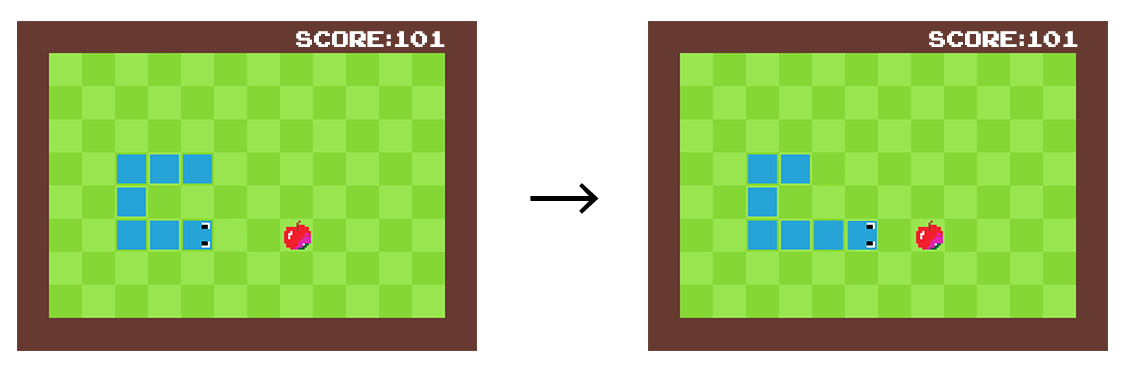
\includegraphics[width = \linewidth]{img/snake.png}
\end{center}

In this question, you will make use of the list node class `\ttt{Node}' defined below to implement several operations of the doubly-linked-list in C++ to support this game.

\begin{cpp}
    struct Node {
      int x, y;
      Node *prev, *next;
      Node(int _x, int _y, Node *_prev, Node *_next)
    	  : x(_x), y(_y), prev(_prev), next(_next) {}
    };
    Node *head, *tail;
\end{cpp}

Please pay attention to the following rules.

\begin{itemize}
	\item Use \bluett{new} and \bluett{delete} to deal with memory issues.
	\item Use \bluett{nullptr} (instead of \bluett{NULL}) for null pointer value.
	\item Make sure your code \textbf{compiles} and does not cause \textbf{runtime-errors} or \textbf{memory-leaks}.
	\item You can fill in each blank line with at most one statement. You don't have to use all of the blank lines.
	\item For simplicity, you can directly access node attributes like \ttt{node->prev}, \ttt{node->next}, etc. This is not recommended for practical programming but OK for this question.
\end{itemize}

\pagebreak

\begin{parts}
	\part[5] \textbf{Update the Snake Head}\par
	We want to create a new node to store the new location of the snake head, and insert it before the original head. You may assume that the snake has at least two nodes. Please fill in the blanks below.
	%%%%%%%%%%%%%%%%%%%%%%%%%%%%%%%%%%%%%%%%%%%%%%%%%%%%%%%%%%%%%%%%%%%%%%
	% Replace '____________' below with your code!
	%%%%%%%%%%%%%%%%%%%%%%%%%%%%%%%%%%%%%%%%%%%%%%%%%%%%%%%%%%%%%%%%%%%%%%
	\linespread{1.5}
	\begin{cpp}
void update_head(int x, int y) {
  Node *new_head = new Node(x, y, nullptr, head);
  head->prev = new_head;
  head = new_head;
}
	\end{cpp}
	\linespread{1}
	\part[5] \textbf{Remove the Snake Tail}\par
	We want to remove the tail node of the snake and update the information of the tail. You may assume that the snake has at least two nodes. Please fill in the blanks below.
	%%%%%%%%%%%%%%%%%%%%%%%%%%%%%%%%%%%%%%%%%%%%%%%%%%%%%%%%%%%%%%%%%%%%%%
	% Replace '____________' below with your code!
	%%%%%%%%%%%%%%%%%%%%%%%%%%%%%%%%%%%%%%%%%%%%%%%%%%%%%%%%%%%%%%%%%%%%%%
	\linespread{1.5}
	\begin{cpp}
void remove_tail() {
  Node *old_tail = tail;
  tail = tail->prev;
  tail->next = nullptr;
  delete old_tail;
}
	\end{cpp}
	\linespread{1}

	\part[2] \textbf{Eat the Fruit}\par
	If the snake head would touch the fruit at \((x,y)\) after a certain step, the snake will eat the fruit and increase its length by one node. Then for this step, which of the following operations should we call? Tick (\(\surd\)) the correct answer.

	%%%%%%%%%%%%%%%%%%%%%%%%%%%%%%%%%%%%%%%%%%%%%%%%%%%%%%%%%%%%%%%%%%%%%%
	% Replace `\choice' with `\CorrectChoice' on the selected choice!
	%%%%%%%%%%%%%%%%%%%%%%%%%%%%%%%%%%%%%%%%%%%%%%%%%%%%%%%%%%%%%%%%%%%%%%
	\begin{checkboxes}
		\choice \ttt{remove\_tail()}
		\CorrectChoice \ttt{update\_head(x, y)}
		\choice \ttt{update\_head(x, y)} and \ttt{remove\_tail()}
	\end{checkboxes}
\end{parts}

\newpage

\titledquestion{Let's Play with Linked-List, Stack and Queue}

In the following questions, we want to implement the \ttt{push} and \ttt{pop} operations of stacks and queues with singly-linked-lists in the most efficient way. You can only access the head node of the linked-list. Access to the tail node is not allowed.

You can answer this question using pseudocode or natural language. Please make sure your description is clear and easy to understand.

\begin{parts}
	\part[5]\label{part:5a} \textbf{Stack Using Linked-List}\par
	Please specify how you implement stack's \ttt{push} and \ttt{pop} operations.
	\begin{solution}
		%%%%%%%%%%%%%%%%%%%%%%%%%%%%%%%%%%%%%%%%%%%%%%%%%%%%%%%%%%%%%
		% Replace the `vspace{2.5in}' with your answer.
		%%%%%%%%%%%%%%%%%%%%%%%%%%%%%%%%%%%%%%%%%%%%%%%%%%%%%%%%%%%%%
		%\vspace{2.5in}

		To implement the \ttt{push} and \ttt{pop} operations of stacks by using Linked-List
		
		we need to set a structure called Node, each node contains the some elements that we need to store,
		and a next pointer, points to the node which is the early one to enter the stack 
		
		we also need a head pointer, points to the top node of the stack

		the implement of push operator:
		
		\begin{cpp}
void push(Node* new_element)
{
  Node* new_head = new_element;
  new_head->next = head;
  head = new_element;
}
		\end{cpp}

		for pop operator, one thing needs to notice is that if the stack is empty, we can not execute the pop instruction
		
		so we need to check whether the stack is empty or not before removing the top node of the stack
		
		the implement of pop operator:
		
		\begin{cpp}
int pop()
{
  if(head->next == nullptr)
    return 0;   // the stack is empty, 
			// we failed to execute the pop instruction
  Node* old_head = head;
  head = head->next;
  delete old_head;
  old_head = nullptr;
  return 1;       // the stack is not empty, 
			// we successed to execute the pop instruction
}
		\end{cpp}

	\end{solution}

	\newpage
	
	\part[5] \textbf{Queue Using Linked-Lists}\par
	Please specify how you implement queue's \ttt{push} and \ttt{pop} operations with linked-list operations. You may directly use the operations you implemented in part (\ref{part:5a}).\par
	\emph{\textbf{Hint:} Use multiple stacks to implement a queue.}
	\begin{solution}
		%%%%%%%%%%%%%%%%%%%%%%%%%%%%%%%%%%%%%%%%%%%%%%%%%%%%%%%%%%%%%
		% Replace the `vspace{2.5in}' with your answer.
		%%%%%%%%%%%%%%%%%%%%%%%%%%%%%%%%%%%%%%%%%%%%%%%%%%%%%%%%%%%%%
		%\vspace{2.5in}

		To implement the \ttt{push} and \ttt{pop} operations of queues by using Linked-List
		
		we can use two stacks to implement a queue
		name two stacks A and B (each has their own head pointer: headA ,head B)
		
		for the push implement:

		1. we need to check whether stack B is empty
		   
			if stack B is not empty, we need to remove all the elements in stack B into stack A with the push and pop implments of stacks
		
		2. after stack B becomes empty, we put the new element into stack A

		the implement of push operator:
		
		some part of the function is pseudocode(stackA. means the operations of stack A , stackB. means the operations of stack B)
		
		\begin{cpp}
void push(Node* new_element)
{
  if(headB->next != nullptr)
  {
    while(headB->next != nullptr)
    {
      stackA.push(stackB.top());
      stackB.pop();
    }
  }
  stackA.push(new_element);
}
		\end{cpp}

		for the pop implement:
		
		1. we need to check whether stack A is empty
		   
			if stack A is not empty, we need to remove all the elements in stack A into stack B with the push and pop implments of stacks
		
		
		2. after stack A becomes empty, we need to check whether stack B is empty
			
			a. if stack B is empty, then it means that the queue is empty, so we fail to implement pop operate this time
			
			b. if stack B is not empty, we just need to pop the top element of stack B

		the top() operate means that get the head element of the stack
		
		the implement of pop operator:
		
		some part of the function is pseudocode(stackA. means the operations of stack A , stackB. means the operations of stack B)
		
		\begin{cpp}
int pop()
{
  if(headA->next != nullptr)  // the stackA is not empty, 
  {		    // we need to remove the elements into stackB
    while((headA->next != nullptr)
    {
      stackB.push(stackA.top());
      stackA.pop();
    }
  }
  if(headB->next == nullptr)  // the stackB is empty,
    return 0;   // we failed to execute the pop instruction
  stackB.pop();
  return 1;       // the stackB is not empty, 
	        // we successed to execute the pop instruction
}
		\end{cpp}
	\end{solution}
\end{parts}

\end{questions}

\end{document}